\chapter{DISEÑO DE LA SOLUCIÓN}

El diseño del observatorio de demanda laboral se fundamentó en una arquitectura modular de pipeline lineal, donde cada componente procesa datos de forma secuencial y almacena sus resultados en una base de datos centralizada. Esta arquitectura garantiza la trazabilidad, la escalabilidad y la capacidad de replicar o reejecutar cualquier etapa del proceso de manera independiente.

\section{Contexto del Sistema}

La Figura \ref{fig:contexto-sistema} presenta el diagrama de contexto del observatorio, mostrando los actores externos, sistemas externos y componentes internos principales. Este diagrama, basado en el modelo C4, proporciona una vista de alto nivel de las fronteras del sistema y sus interacciones con el entorno.

\begin{figure}[H]
\centering
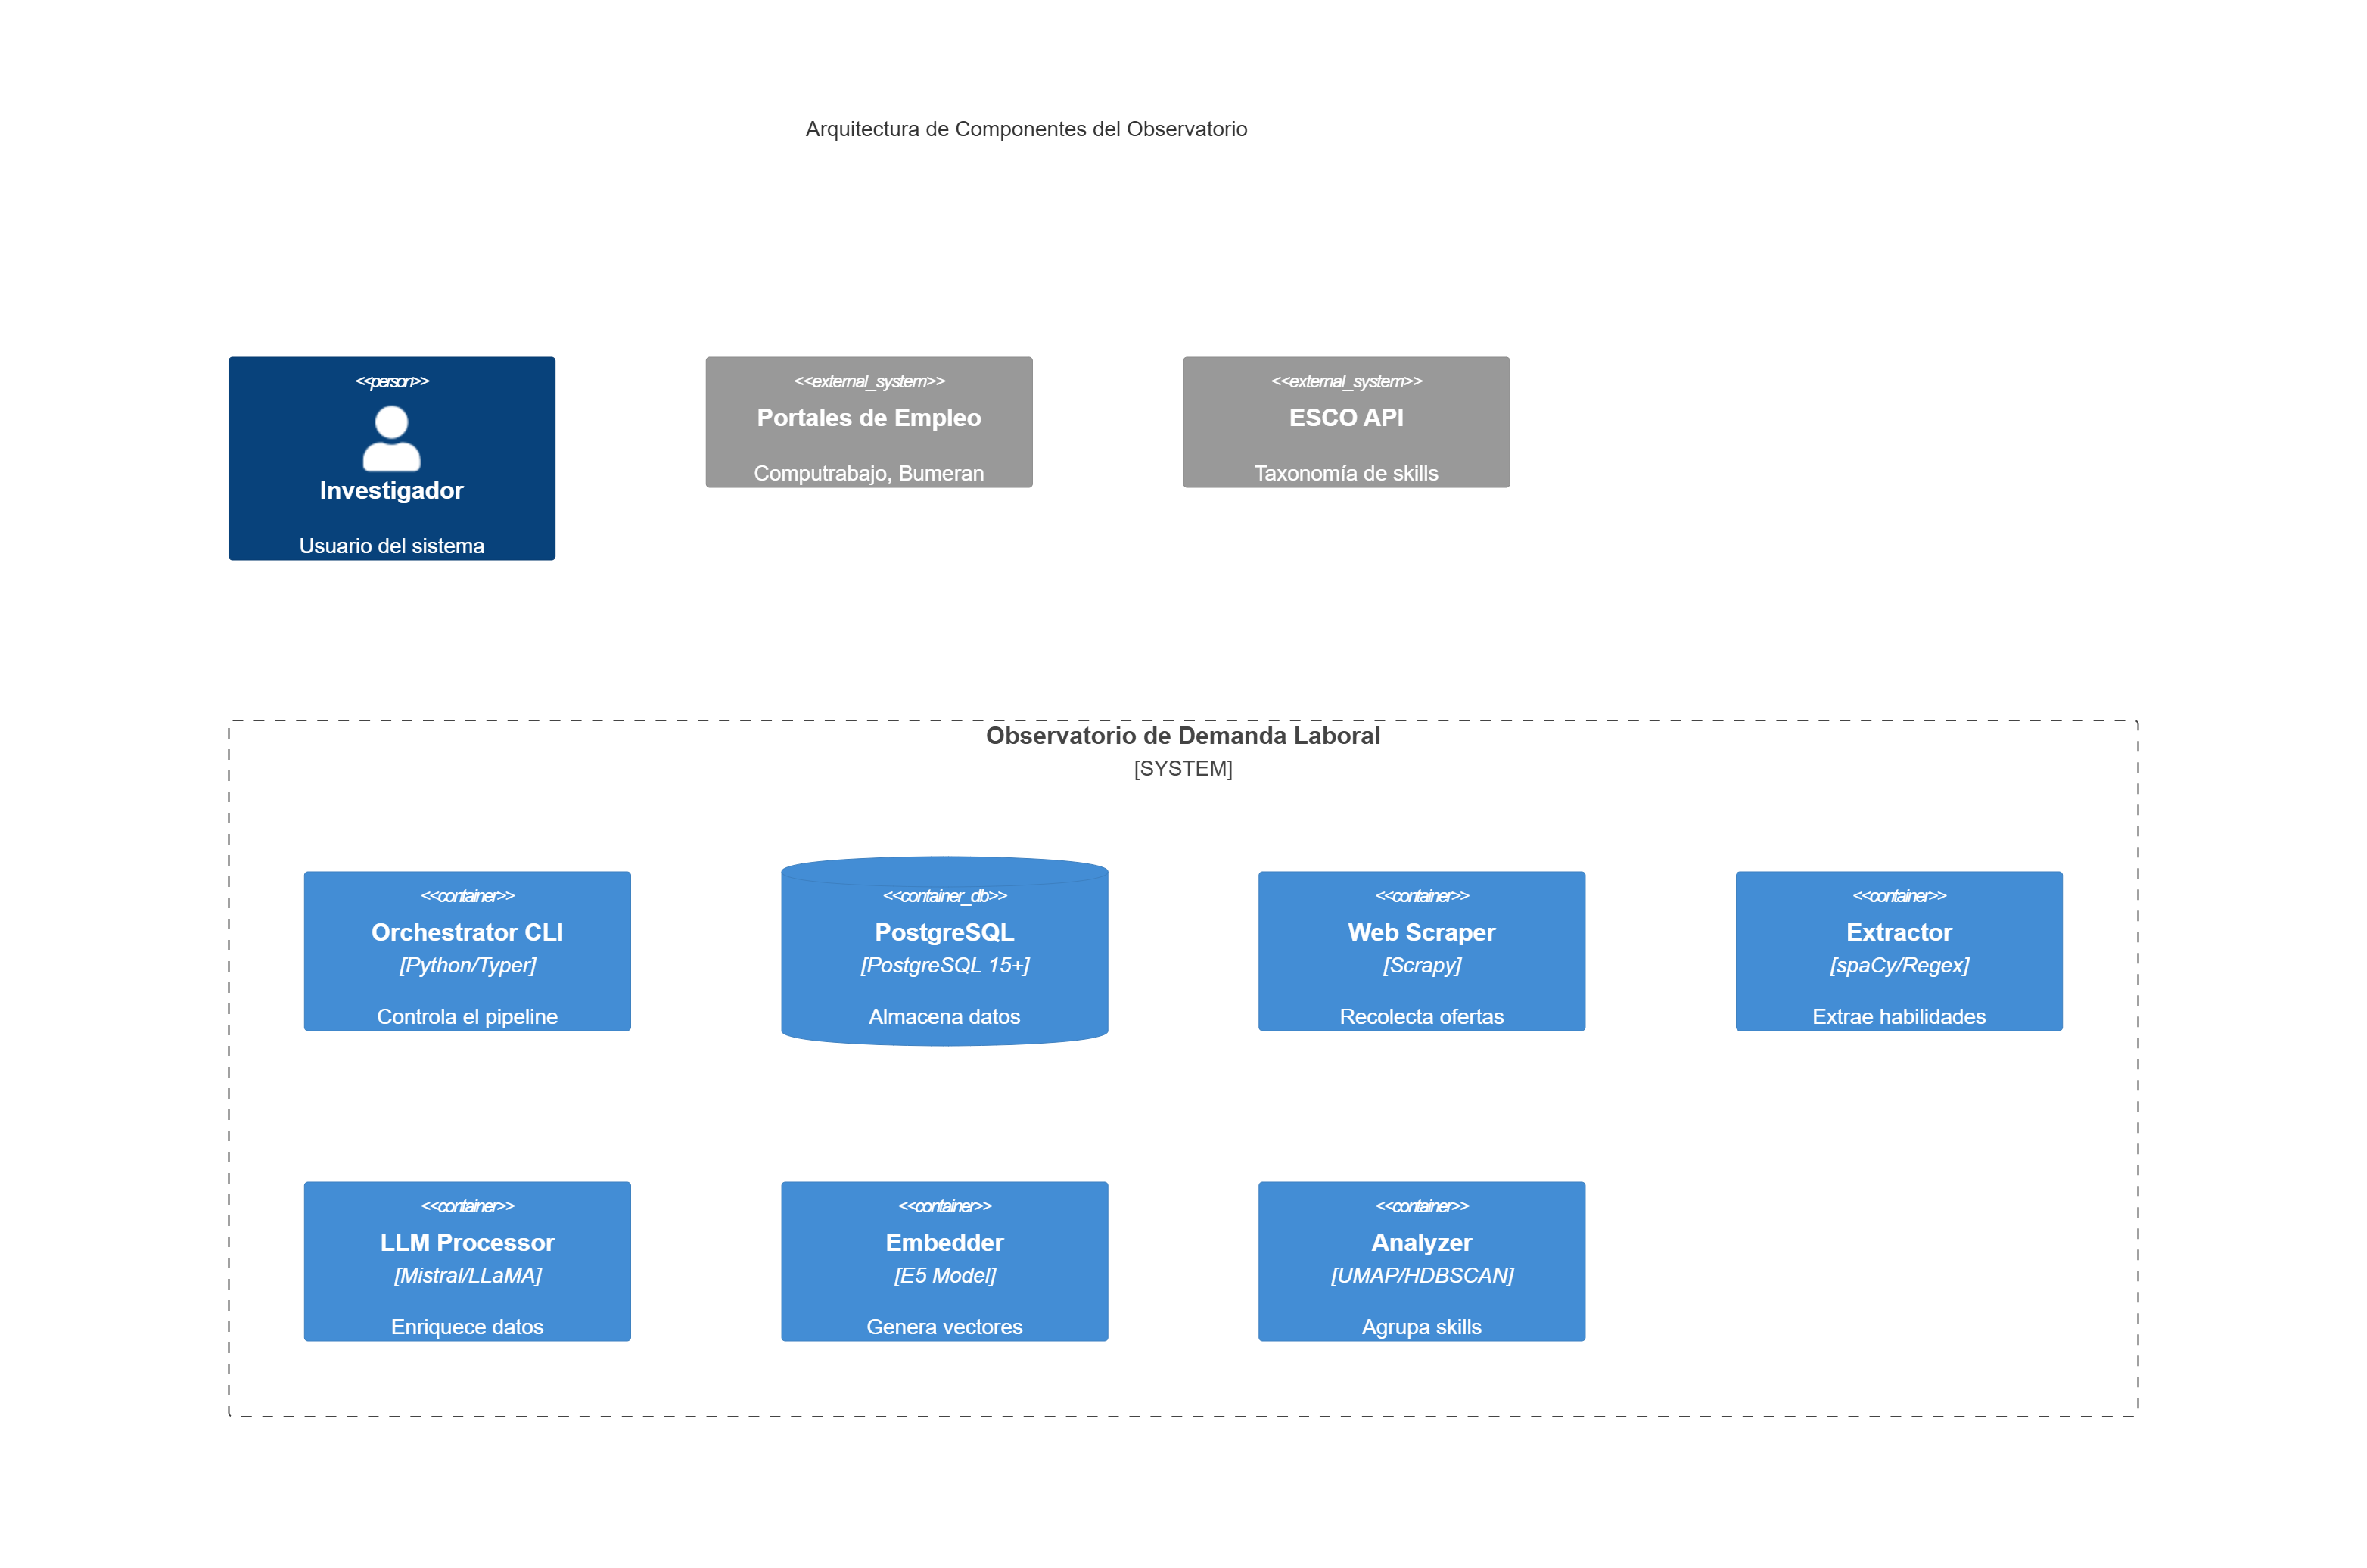
\includegraphics[width=0.95\textwidth]{diagrams/Contexto(Faltan conexiones).png}
\caption{Diagrama de Contexto del Observatorio de Demanda Laboral}
\label{fig:contexto-sistema}
\end{figure}

El sistema interactúa con tres entidades externas principales:

\begin{itemize}
    \item \textbf{Investigador}: Usuario principal del sistema que inicia el proceso de scraping, configura parámetros de análisis y consume los reportes generados.
    \item \textbf{Portales de Empleo}: Fuentes de datos externas (Computrabajo, Bumeran, ElEmpleo) que publican ofertas laborales en formato HTML.
    \item \textbf{ESCO API}: Taxonomía europea de habilidades y competencias utilizada para normalizar y clasificar las habilidades extraídas.
\end{itemize}

Internamente, el sistema está compuesto por siete componentes principales que operan de forma coordinada: Orchestrator CLI (control del pipeline), PostgreSQL (almacenamiento), Web Scraper (adquisición), Extractor (NLP), LLM Processor (enriquecimiento), Embedder (vectorización) y Analyzer (clustering y visualización).

\section{Arquitectura General del Sistema}

\subsection{Pipeline Lineal de 8 Etapas}

El sistema se diseñó como un pipeline secuencial compuesto por ocho módulos especializados que transforman progresivamente los datos brutos en conocimiento estructurado sobre el mercado laboral:

\begin{enumerate}
    \item \textbf{Módulo de Scraping (Scrapy)}: Recolección automatizada de ofertas laborales desde portales web.
    \item \textbf{Módulo de Extracción (NER + Regex)}: Identificación de habilidades explícitas mediante reconocimiento de entidades y patrones.
    \item \textbf{Módulo LLM (Mistral/LLaMA)}: Enriquecimiento semántico y detección de habilidades implícitas.
    \item \textbf{Módulo de Embeddings (E5 Multilingüe)}: Generación de representaciones vectoriales de habilidades.
    \item \textbf{Módulo de Reducción Dimensional (UMAP)}: Proyección a espacios de baja dimensionalidad.
    \item \textbf{Módulo de Clustering (HDBSCAN)}: Agrupamiento no supervisado de habilidades.
    \item \textbf{Módulo de Visualización}: Generación de gráficos y páginas web estáticas.
    \item \textbf{Módulo de Reportes}: Exportación de resultados en formato PDF, PNG y CSV.
\end{enumerate}

\subsection{Representación Visual de la Arquitectura}

La arquitectura del observatorio se presenta desde tres perspectivas complementarias que permiten comprender el sistema en su totalidad: la vista modular detallada, la vista por capas de responsabilidad y la vista de transformación de datos.

\subsubsection{Vista Modular: Pipeline de 8 Etapas}

La Figura \ref{fig:arquitectura-completa} presenta la arquitectura modular completa del sistema, detallando cada una de las ocho etapas del pipeline con sus tecnologías específicas, funciones, entradas, salidas y mecanismos de almacenamiento. Esta vista es fundamental para comprender la responsabilidad individual de cada módulo y cómo estos se integran para formar el sistema completo.

\begin{figure}[H]
\centering
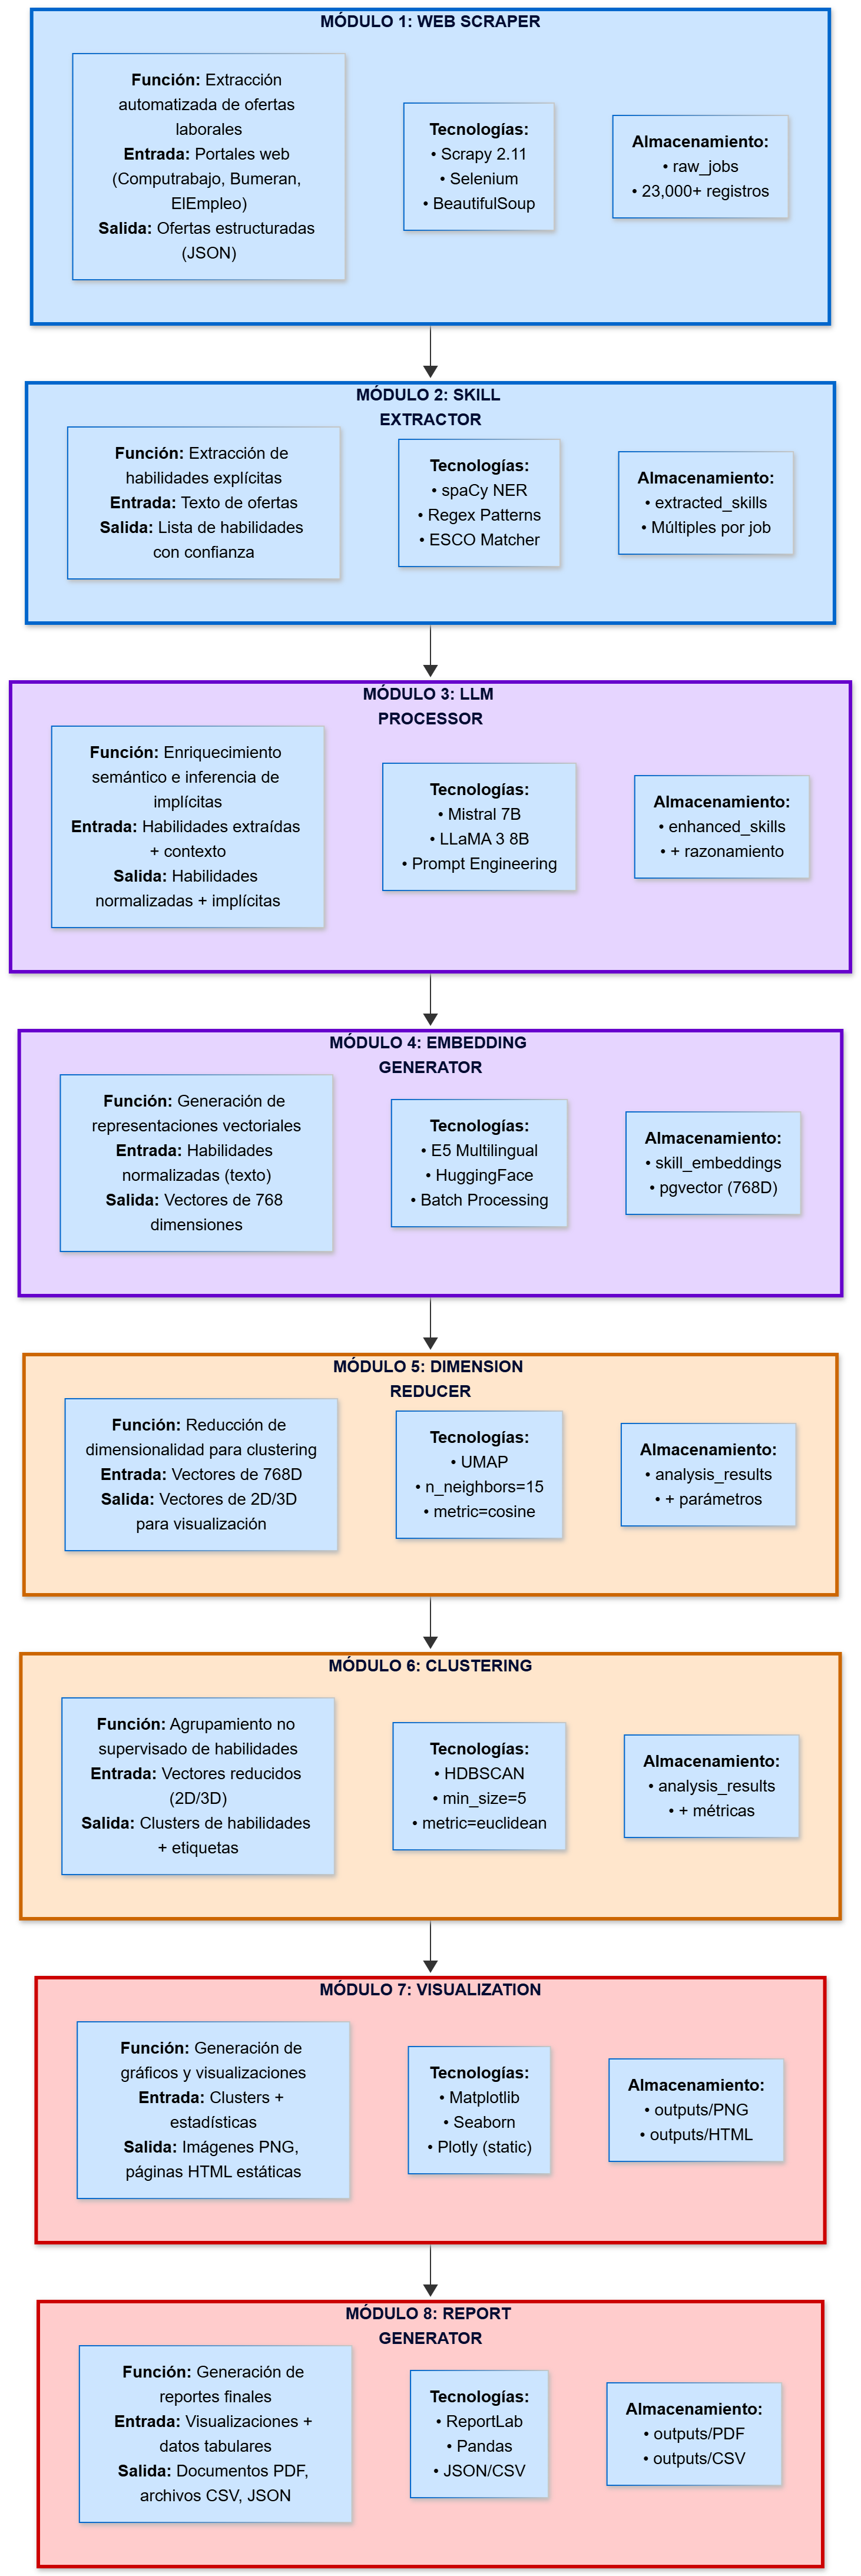
\includegraphics[width=0.45\textwidth]{diagrams/ArquitecturaGeneral.png}
\caption{Arquitectura Modular Completa del Observatorio - Pipeline de 8 Etapas}
\label{fig:arquitectura-completa}
\end{figure}

Cada módulo del pipeline opera de forma autónoma y puede ser ejecutado independientemente, lo que facilita el desarrollo incremental, las pruebas unitarias y la depuración. Los módulos 1-2 se enfocan en la adquisición y extracción inicial de datos; los módulos 3-4 realizan el enriquecimiento semántico mediante inteligencia artificial; los módulos 5-6 ejecutan el análisis no supervisado; y finalmente, los módulos 7-8 generan las salidas consumibles por usuarios finales.

\subsubsection{Vista por Capas: Separación de Responsabilidades}

La Figura \ref{fig:arquitectura-capas} reorganiza los componentes del sistema en siete capas lógicas, mostrando cómo se distribuyen las responsabilidades y cómo fluye el control y los datos entre capas. Esta representación es especialmente útil para comprender la arquitectura desde una perspectiva de ingeniería de software y para identificar las dependencias entre componentes.

\begin{figure}[H]
\centering
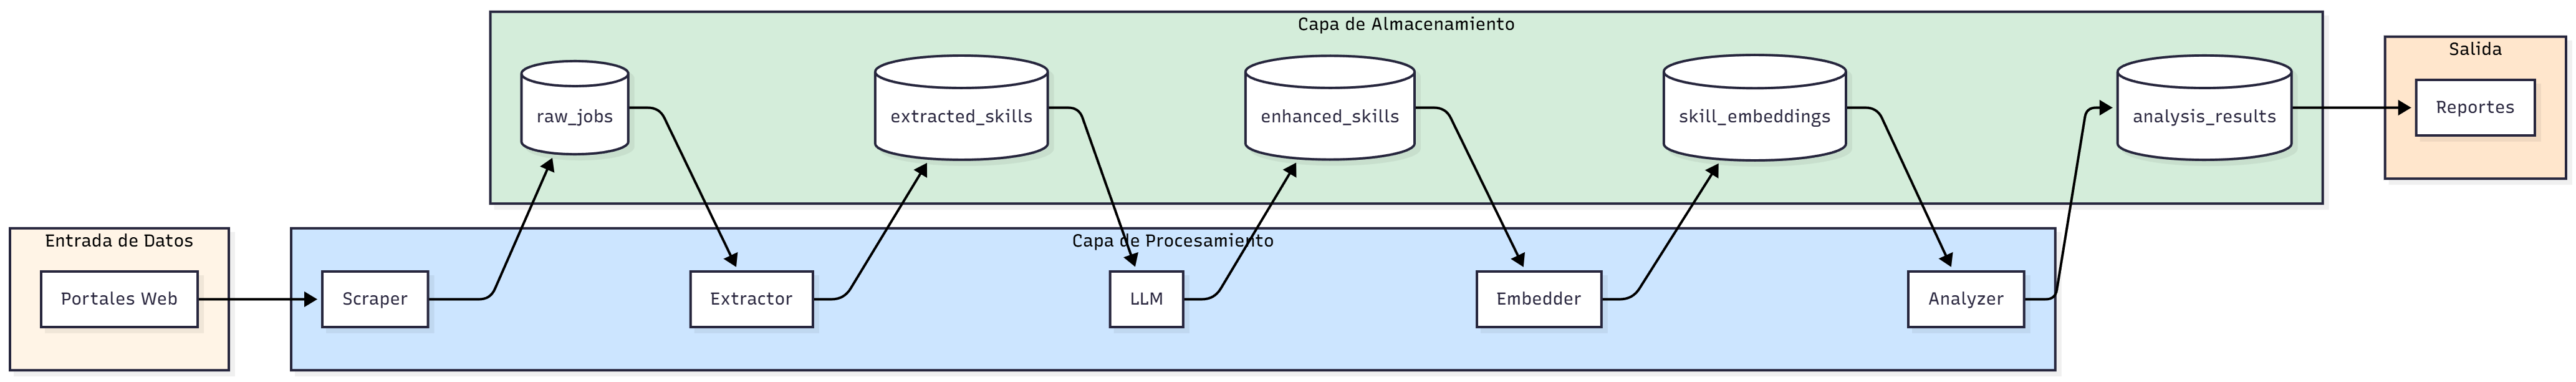
\includegraphics[width=0.95\textwidth]{diagrams/ArquitecturaHorizontal.png}
\caption{Arquitectura en Capas del Sistema - Vista de Separación de Responsabilidades}
\label{fig:arquitectura-capas}
\end{figure}

Las capas 1-5 representan el flujo vertical de procesamiento de datos (de arriba hacia abajo), mientras que la capa 6 (Persistencia) actúa como el repositorio central al que todas las capas superiores acceden para lectura y escritura. La capa 7 (Orquestación) coordina transversalmente la ejecución de todas las demás capas, implementando el patrón de orquestador que controla el ciclo de vida completo del sistema.

\subsubsection{Vista de Estados: Ciclo de Vida de Jobs}

La Figura \ref{fig:estados-jobs} ilustra el ciclo de vida completo que atraviesan las ofertas laborales desde su ingreso al sistema hasta la generación de reportes. Este diagrama de estados muestra las transiciones entre las diferentes etapas de procesamiento, incluyendo los caminos de manejo de errores y reintentos.

\begin{figure}[H]
\centering
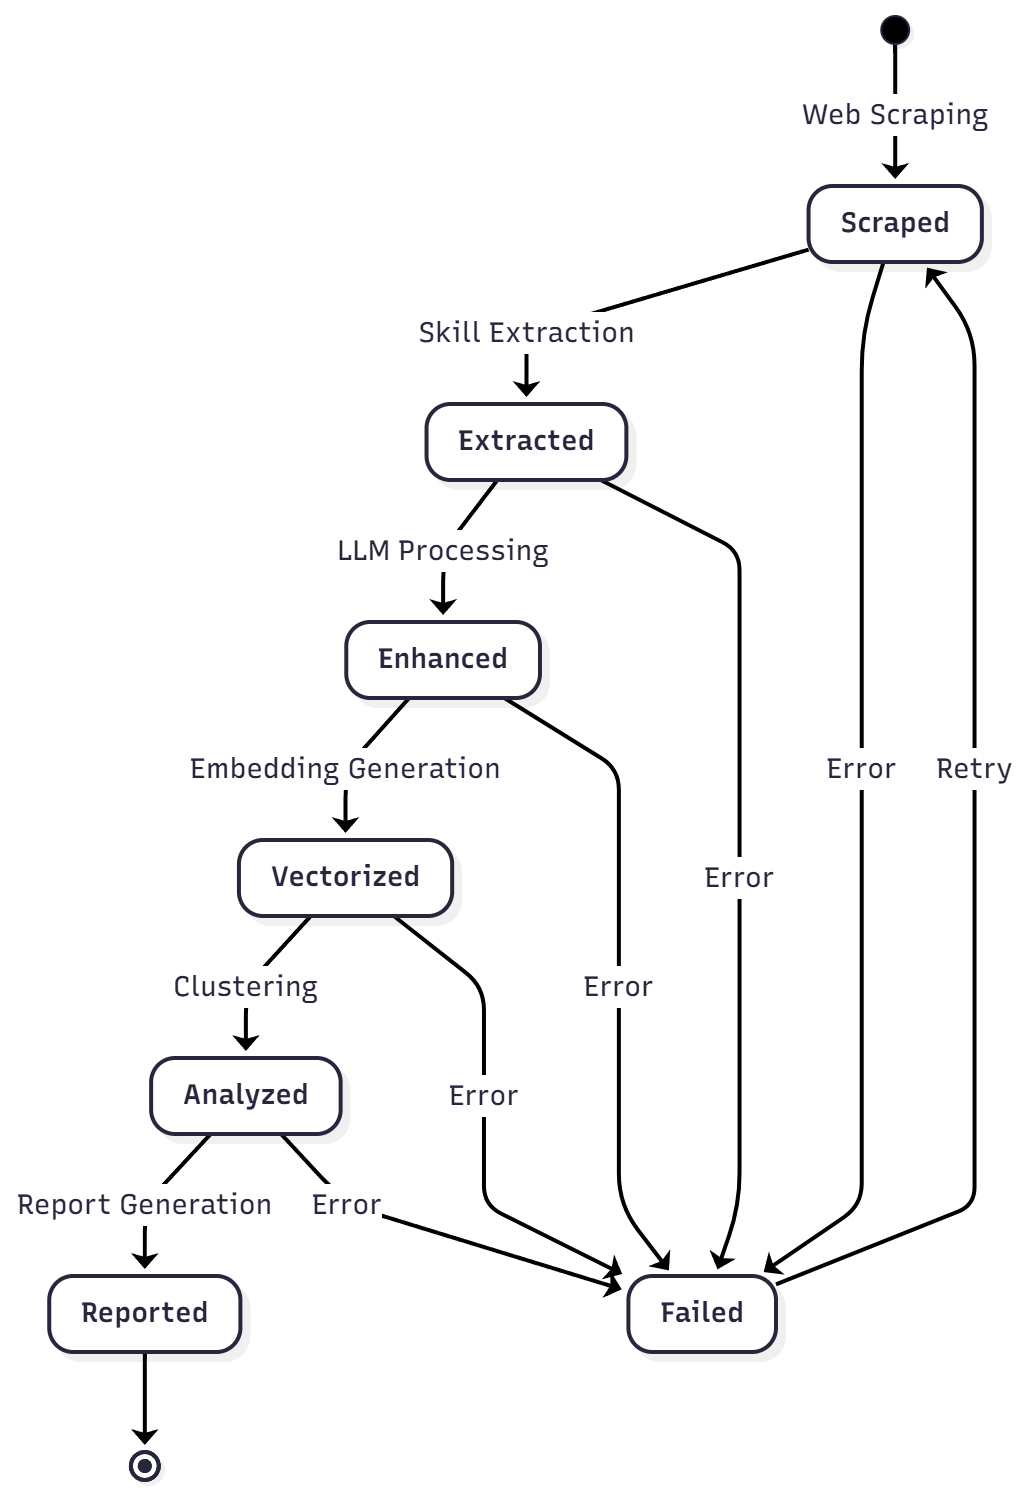
\includegraphics[width=0.6\textwidth]{diagrams/DiagramaEstado.png}
\caption{Diagrama de Estados del Procesamiento de Ofertas Laborales}
\label{fig:estados-jobs}
\end{figure}

Como se observa, los datos atraviesan seis estados principales: \textbf{Scraped} $\rightarrow$ \textbf{Extracted} $\rightarrow$ \textbf{Enhanced} $\rightarrow$ \textbf{Vectorized} $\rightarrow$ \textbf{Analyzed} $\rightarrow$ \textbf{Reported}. En cada transición, el sistema puede detectar errores que llevan al estado \textbf{Failed}, desde donde se pueden aplicar reintentos automáticos. Esta arquitectura de estados garantiza la trazabilidad completa y la capacidad de recuperación ante fallos en cualquier etapa del pipeline.

\section{Diseño de la Base de Datos}

La arquitectura de datos se sustenta en PostgreSQL 15+, seleccionado por su robustez, soporte JSON nativo y capacidad de extensión mediante pgvector para operaciones de similitud vectorial.

\subsection{Esquema de la Base de Datos}

La base de datos está compuesta por seis tablas principales que capturan el flujo completo del pipeline:

\subsubsection{Tabla: raw\_jobs}

Almacena las ofertas laborales tal como fueron extraídas de los portales web:

\begin{verbatim}
CREATE TABLE raw_jobs (
    job_id UUID PRIMARY KEY,
    portal VARCHAR(50) NOT NULL,
    country CHAR(2) NOT NULL,
    url TEXT NOT NULL,
    title TEXT NOT NULL,
    company TEXT,
    location TEXT,
    description TEXT NOT NULL,
    requirements TEXT,
    salary_raw TEXT,
    contract_type VARCHAR(50),
    remote_type VARCHAR(50),
    posted_date DATE,
    scraped_at TIMESTAMP DEFAULT CURRENT_TIMESTAMP,
    content_hash VARCHAR(64) UNIQUE,
    is_processed BOOLEAN DEFAULT FALSE
);
\end{verbatim}

\textbf{Campos clave}:
\begin{itemize}
    \item \texttt{job\_id}: Identificador único generado con UUID v4
    \item \texttt{portal}: Origen de la oferta (computrabajo, bumeran, elempleo)
    \item \texttt{country}: Código ISO 3166-1 alpha-2 (CO, MX, AR)
    \item \texttt{content\_hash}: Hash SHA-256 del contenido para detección de duplicados
    \item \texttt{is\_processed}: Bandera de control para procesamiento incremental
\end{itemize}

\subsubsection{Tabla: extracted\_skills}

Contiene las habilidades identificadas mediante técnicas de NER y expresiones regulares:

\begin{verbatim}
CREATE TABLE extracted_skills (
    extraction_id UUID PRIMARY KEY,
    job_id UUID REFERENCES raw_jobs(job_id),
    skill_text TEXT NOT NULL,
    skill_type VARCHAR(50),
    extraction_method VARCHAR(50),
    confidence_score FLOAT,
    source_section VARCHAR(50),
    span_start INTEGER,
    span_end INTEGER,
    esco_uri TEXT,
    extracted_at TIMESTAMP DEFAULT CURRENT_TIMESTAMP
);
\end{verbatim}

\textbf{Campos clave}:
\begin{itemize}
    \item \texttt{extraction\_method}: Indica el método de extracción (ner, regex, esco\_match)
    \item \texttt{confidence\_score}: Nivel de confianza de la extracción (0-1)
    \item \texttt{source\_section}: Sección de origen (title, description, requirements)
    \item \texttt{span\_start/span\_end}: Posición del span en el texto original
    \item \texttt{esco\_uri}: Enlace a la taxonomía ESCO cuando existe correspondencia
\end{itemize}

\subsubsection{Tabla: enhanced\_skills}

Almacena las habilidades enriquecidas por el procesamiento LLM:

\begin{verbatim}
CREATE TABLE enhanced_skills (
    enhancement_id UUID PRIMARY KEY,
    job_id UUID REFERENCES raw_jobs(job_id),
    original_skill_text TEXT,
    normalized_skill TEXT NOT NULL,
    skill_type VARCHAR(50),
    esco_concept_uri TEXT,
    esco_preferred_label TEXT,
    llm_confidence FLOAT,
    llm_reasoning TEXT,
    is_duplicate BOOLEAN DEFAULT FALSE,
    duplicate_of_id UUID,
    enhanced_at TIMESTAMP DEFAULT CURRENT_TIMESTAMP,
    llm_model VARCHAR(100)
);
\end{verbatim}

\textbf{Campos clave}:
\begin{itemize}
    \item \texttt{normalized\_skill}: Versión normalizada de la habilidad según ESCO
    \item \texttt{skill\_type}: Tipo de habilidad (explicit, implicit, normalized)
    \item \texttt{llm\_confidence}: Confianza del modelo LLM en la inferencia
    \item \texttt{llm\_reasoning}: Justificación del modelo para habilidades implícitas
    \item \texttt{is\_duplicate}: Bandera para habilidades duplicadas identificadas
\end{itemize}

\subsubsection{Tabla: skill\_embeddings}

Contiene las representaciones vectoriales de las habilidades:

\begin{verbatim}
CREATE TABLE skill_embeddings (
    embedding_id UUID PRIMARY KEY,
    skill_text TEXT UNIQUE NOT NULL,
    embedding vector(768) NOT NULL,
    model_name VARCHAR(100) NOT NULL,
    model_version VARCHAR(50),
    created_at TIMESTAMP DEFAULT CURRENT_TIMESTAMP
);

CREATE INDEX ON skill_embeddings
USING ivfflat (embedding vector_cosine_ops)
WITH (lists = 100);
\end{verbatim}

\textbf{Características}:
\begin{itemize}
    \item Utiliza la extensión \texttt{pgvector} para almacenar vectores de 768 dimensiones
    \item Implementa índice IVFFlat para búsquedas de similitud eficientes
    \item Los vectores son generados con el modelo E5 multilingüe
    \item Soporte para operaciones de distancia coseno
\end{itemize}

\subsubsection{Tabla: analysis\_results}

Almacena los resultados de análisis de clustering y tendencias:

\begin{verbatim}
CREATE TABLE analysis_results (
    analysis_id UUID PRIMARY KEY,
    analysis_type VARCHAR(50),
    country CHAR(2),
    date_range_start DATE,
    date_range_end DATE,
    parameters JSONB,
    results JSONB,
    created_at TIMESTAMP DEFAULT CURRENT_TIMESTAMP
);
\end{verbatim}

\textbf{Campos clave}:
\begin{itemize}
    \item \texttt{analysis\_type}: Tipo de análisis (clustering, trends, profile)
    \item \texttt{parameters}: Configuración del análisis en formato JSON
    \item \texttt{results}: Resultados estructurados en formato JSON
    \item Uso de tipo de datos JSONB para flexibilidad y eficiencia en consultas
\end{itemize}

\subsubsection{Tabla: esco\_skills}

Contiene la taxonomía ESCO completa con más de 13,000 habilidades:

\begin{verbatim}
CREATE TABLE esco_skills (
    esco_uri TEXT PRIMARY KEY,
    preferred_label_es TEXT NOT NULL,
    preferred_label_en TEXT,
    alt_labels TEXT[],
    skill_type VARCHAR(50),
    description TEXT,
    skill_reuse_level VARCHAR(50),
    last_updated TIMESTAMP
);
\end{verbatim}

\textbf{Características}:
\begin{itemize}
    \item Integración completa de la taxonomía ESCO v1.1.0
    \item Soporte multilingüe (español e inglés)
    \item Almacenamiento de etiquetas alternativas como array
    \item Metadatos sobre el nivel de reutilización de la habilidad
\end{itemize}

\subsection{Modelo Entidad-Relación}

La Figura \ref{fig:diagrama-er} presenta el modelo entidad-relación completo de la base de datos, mostrando las cinco tablas principales del pipeline y sus relaciones con la tabla de referencia ESCO. Este diagrama ilustra claramente el flujo de datos entre tablas y las dependencias mediante llaves foráneas.

\begin{figure}[H]
\centering
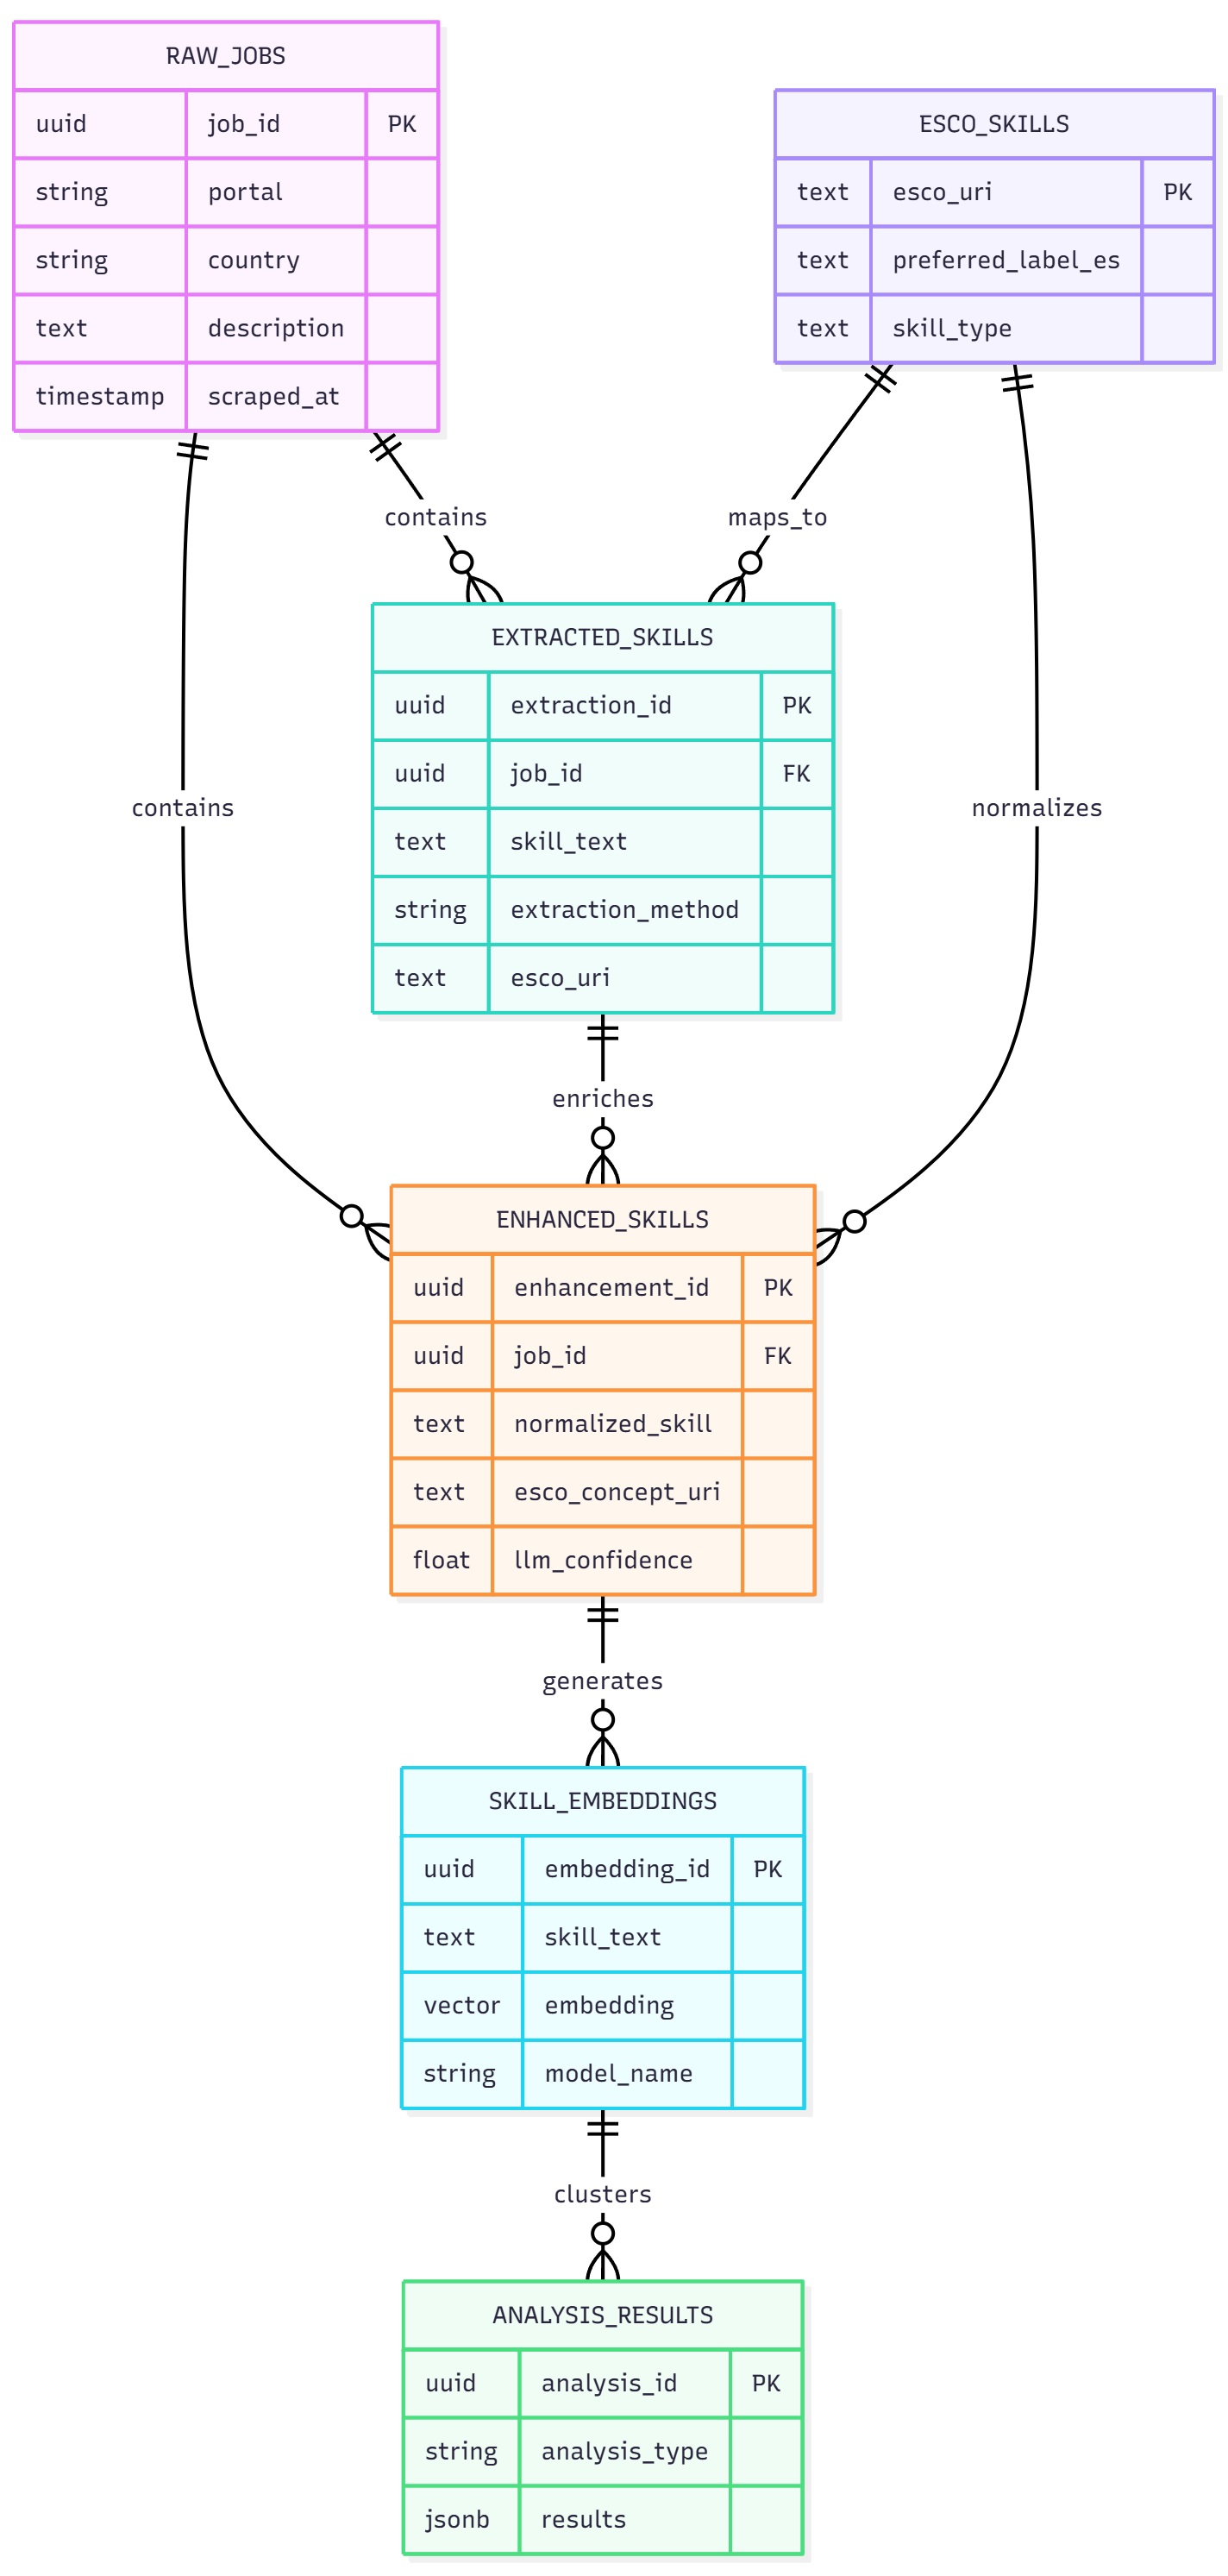
\includegraphics[width=0.5\textwidth]{diagrams/DiagramaER.png}
\caption{Diagrama Entidad-Relación de la Base de Datos del Observatorio}
\label{fig:diagrama-er}
\end{figure}

El modelo de datos sigue una arquitectura de pipeline lineal donde cada tabla representa una etapa de procesamiento:

\begin{itemize}
    \item \texttt{raw\_jobs} es el punto de entrada y contiene referencias (FK) en todas las tablas derivadas
    \item \texttt{extracted\_skills} enriquece (\textit{enriches}) a \texttt{enhanced\_skills}
    \item \texttt{enhanced\_skills} genera (\textit{generates}) vectores en \texttt{skill\_embeddings}
    \item \texttt{skill\_embeddings} alimenta (\textit{clusters}) los resultados en \texttt{analysis\_results}
    \item \texttt{esco\_skills} actúa como tabla de referencia normalizada mediante mapeos desde \texttt{extracted\_skills} y \texttt{enhanced\_skills}
\end{itemize}

Esta arquitectura garantiza integridad referencial y permite trazabilidad completa desde cualquier resultado de análisis hasta la oferta laboral original.

\section{Especificación de Módulos}

\subsection{Módulo 1: Web Scraper}

\textbf{Propósito}: Recolección automatizada de ofertas laborales desde portales de empleo en Colombia, México y Argentina.

\textbf{Tecnologías}:
\begin{itemize}
    \item \textbf{Scrapy 2.11}: Framework asíncrono para scraping a gran escala
    \item \textbf{Selenium + ChromeDriver}: Para portales con contenido dinámico
    \item \textbf{BeautifulSoup 4.12}: Parsing y extracción de HTML
\end{itemize}

\textbf{Características clave}:
\begin{itemize}
    \item Scraping concurrente con límites de tasa por portal
    \item Rotación de user-agents y delays adaptativos
    \item Detección de duplicados mediante hashing de contenido
    \item Reintentos con backoff exponencial ante fallos
    \item Manejo de paginación automática
\end{itemize}

\textbf{Portales soportados}:
\begin{itemize}
    \item Computrabajo (CO, MX, AR)
    \item Bumeran (MX, AR)
    \item ElEmpleo (CO)
    \item InfoJobs (MX)
    \item OCC Mundial (MX)
    \item ZonaJobs (AR)
\end{itemize}

\subsection{Módulo 2: Skill Extractor}

\textbf{Propósito}: Extracción de habilidades explícitas mediante técnicas de NLP.

\textbf{Componentes}:

\begin{enumerate}
    \item \textbf{NER Extractor}: Utiliza spaCy con el modelo \texttt{es\_core\_news\_lg} y un EntityRuler personalizado poblado con la taxonomía ESCO completa para reconocer entidades de tipo skill/technology.

    \item \textbf{Regex Patterns}: Conjunto de expresiones regulares especializadas para capturar tecnologías con nomenclatura específica (ej. ``Node.js'', ``React.js'', ``Python 3.x'').

    \item \textbf{ESCO Matcher}: Módulo de mapeo que normaliza las habilidades extraídas contra la taxonomía ESCO mediante:
    \begin{itemize}
        \item Coincidencia exacta (case-insensitive)
        \item Coincidencia difusa con umbral de similitud
        \item Búsqueda en etiquetas alternativas
    \end{itemize}
\end{enumerate}

\textbf{Pipeline de procesamiento}:
\begin{verbatim}
1. Concatenar: title + description + requirements
2. Preprocesamiento: limpieza y normalización de texto
3. Extracción NER: identificar entidades con EntityRuler
4. Extracción Regex: aplicar patrones de tecnologías
5. Deduplicación: eliminar menciones repetidas
6. Mapeo ESCO: normalizar contra taxonomía
7. Persistencia: almacenar en extracted_skills
\end{verbatim}

\subsection{Módulo 3: LLM Processor}

\textbf{Propósito}: Enriquecimiento semántico de habilidades y detección de competencias implícitas.

\textbf{Modelos soportados}:
\begin{itemize}
    \item \textbf{Mistral 7B Instruct}: Modelo local mediante llama-cpp-python (cuantización Q4)
    \item \textbf{LLaMA 3 8B}: Alternativa con mejor rendimiento en español
    \item \textbf{OpenAI GPT-4}: Fallback opcional mediante API
\end{itemize}

\textbf{Tareas del módulo}:
\begin{enumerate}
    \item \textbf{Deduplicación inteligente}: Identificar variantes de la misma habilidad (``React'', ``React.js'', ``ReactJS'')
    \item \textbf{Inferencia de habilidades implícitas}: Detectar competencias no mencionadas explícitamente pero requeridas por el contexto del cargo
    \item \textbf{Normalización con ESCO}: Mapear todas las habilidades a conceptos ESCO con confianza
    \item \textbf{Razonamiento explicable}: Generar justificaciones para habilidades implícitas
\end{enumerate}

\textbf{Prompt Engineering}: Se diseñaron prompts específicos para el contexto latinoamericano que incluyen:
\begin{itemize}
    \item Instrucciones para manejar ``Spanglish'' (términos técnicos en inglés en contexto español)
    \item Few-shot examples con ofertas laborales reales de la región
    \item Restricción a la taxonomía ESCO para salidas estructuradas
    \item Solicitud de formato JSON con campos definidos
\end{itemize}

\subsection{Módulo 4: Embedding Generator}

\textbf{Propósito}: Generar representaciones vectoriales semánticas de habilidades.

\textbf{Modelo}: \texttt{intfloat/multilingual-e5-base}
\begin{itemize}
    \item Modelo de embeddings multilingüe de 768 dimensiones
    \item Entrenado específicamente para similitud semántica
    \item Soporte nativo para español e inglés en el mismo espacio vectorial
\end{itemize}

\textbf{Proceso}:
\begin{verbatim}
1. Cargar modelo E5 desde Hugging Face
2. Preprocesar: añadir prefijo "query: " según especificación E5
3. Generar embeddings por lotes (batch_size=32)
4. Normalizar vectores (L2 normalization)
5. Almacenar en PostgreSQL con pgvector
6. Crear índice IVFFlat para búsquedas eficientes
\end{verbatim}

\subsection{Módulo 5: Analyzer}

\textbf{Propósito}: Descubrir patrones y clústeres de habilidades mediante análisis no supervisado.

\textbf{Componentes}:

\subsubsection{Reducción de Dimensionalidad (UMAP)}

\textbf{UMAP (Uniform Manifold Approximation and Projection)}:
\begin{itemize}
    \item Reduce los vectores de 768 dimensiones a 2-3 dimensiones
    \item Preserva tanto estructura local como global
    \item Parámetros clave:
    \begin{itemize}
        \item \texttt{n\_neighbors=15}: Balance entre estructura local y global
        \item \texttt{min\_dist=0.1}: Compactación de puntos cercanos
        \item \texttt{metric='cosine'}: Métrica de similitud
    \end{itemize}
\end{itemize}

\subsubsection{Clustering (HDBSCAN)}

\textbf{HDBSCAN (Hierarchical Density-Based Spatial Clustering)}:
\begin{itemize}
    \item Algoritmo de clustering basado en densidad
    \item No requiere especificar número de clústeres
    \item Identifica ruido automáticamente
    \item Parámetros clave:
    \begin{itemize}
        \item \texttt{min\_cluster\_size=5}: Tamaño mínimo de clúster válido
        \item \texttt{min\_samples=3}: Puntos mínimos para densidad
        \item \texttt{metric='euclidean'}: Post-reducción dimensional
    \end{itemize}
\end{itemize}

\subsubsection{Visualización}

Generación de gráficos estáticos:
\begin{itemize}
    \item Scatter plots 2D/3D de clústeres con matplotlib
    \item Distribuciones de frecuencia de habilidades
    \item Heatmaps de co-ocurrencia de habilidades
    \item Gráficos de barras por país y portal
\end{itemize}

\subsubsection{Generación de Reportes}

Exportación multi-formato:
\begin{itemize}
    \item \textbf{PDF}: Reportes completos con ReportLab incluyendo:
    \begin{itemize}
        \item Resumen ejecutivo de hallazgos
        \item Estadísticas descriptivas
        \item Visualizaciones embebidas
        \item Tablas de top skills por clúster
    \end{itemize}
    \item \textbf{PNG}: Imágenes de alta resolución de visualizaciones
    \item \textbf{CSV}: Datos tabulares para análisis externo
    \item \textbf{JSON}: Resultados estructurados para integración
\end{itemize}

\section{Decisiones Técnicas y Justificación}

La siguiente tabla resume las decisiones arquitectónicas clave y su fundamentación:

\begin{longtable}{|p{3.5cm}|p{3.5cm}|p{7cm}|}
\hline
\textbf{Componente} & \textbf{Tecnología} & \textbf{Justificación} \\
\hline
\endfirsthead

\hline
\textbf{Componente} & \textbf{Tecnología} & \textbf{Justificación} \\
\hline
\endhead

\hline
\endfoot

\hline
\endlastfoot

Base de datos & PostgreSQL 15+ & Soporte JSON nativo (JSONB), extensión pgvector para vectores, robustez empresarial, licencia libre (PostgreSQL License). \\
\hline

Taxonomía & ESCO v1.1.0 & Cobertura superior en español (13,000+ skills), etiquetas multilingües, amplia representación de habilidades tecnológicas, respaldo institucional de la Comisión Europea. \\
\hline

Framework de scraping & Scrapy 2.11 & Arquitectura asíncrona para alto rendimiento, manejo robusto de reintentos y errores, middlewares extensibles, amplia comunidad y documentación. \\
\hline

Modelo NLP & spaCy 3.7 + es\_core\_news\_lg & Mejor modelo disponible para español, soporte de EntityRuler para reglas personalizadas, rendimiento optimizado en CPU. \\
\hline

LLM local & Mistral 7B / LLaMA 3 8B & Ejecución local sin dependencia de APIs externas, buen rendimiento en español post-instrucción, cuantización Q4 para reducir requisitos de memoria (4-5 GB RAM). \\
\hline

Modelo de embeddings & intfloat/multilingual-e5-base & Estado del arte en embeddings multilingües, 768 dimensiones balancean expresividad y eficiencia, soporte nativo para español e inglés en espacio compartido. \\
\hline

Algoritmo de clustering & HDBSCAN & No requiere especificar k, identifica ruido, maneja clústeres de densidades variables, jerárquico permite análisis multinivel. \\
\hline

Reducción dimensional & UMAP & Preserva estructura local y global, superior a t-SNE en escalabilidad y reproducibilidad, parámetros interpretables. \\
\hline

Orquestación & Typer CLI & Interface de línea de comandos tipo Git, validación automática de parámetros, ayuda auto-generada, fácil integración con schedulers. \\
\hline

\end{longtable}

\section{Orquestación y Automatización}

\subsection{Flujo de Interacciones entre Componentes}

La Figura \ref{fig:diagrama-secuencia} presenta el diagrama de secuencia que ilustra el flujo completo de interacciones entre los componentes del sistema durante un ciclo de ejecución completo, desde el comando inicial del usuario hasta la generación de reportes finales.

\begin{figure}[H]
\centering
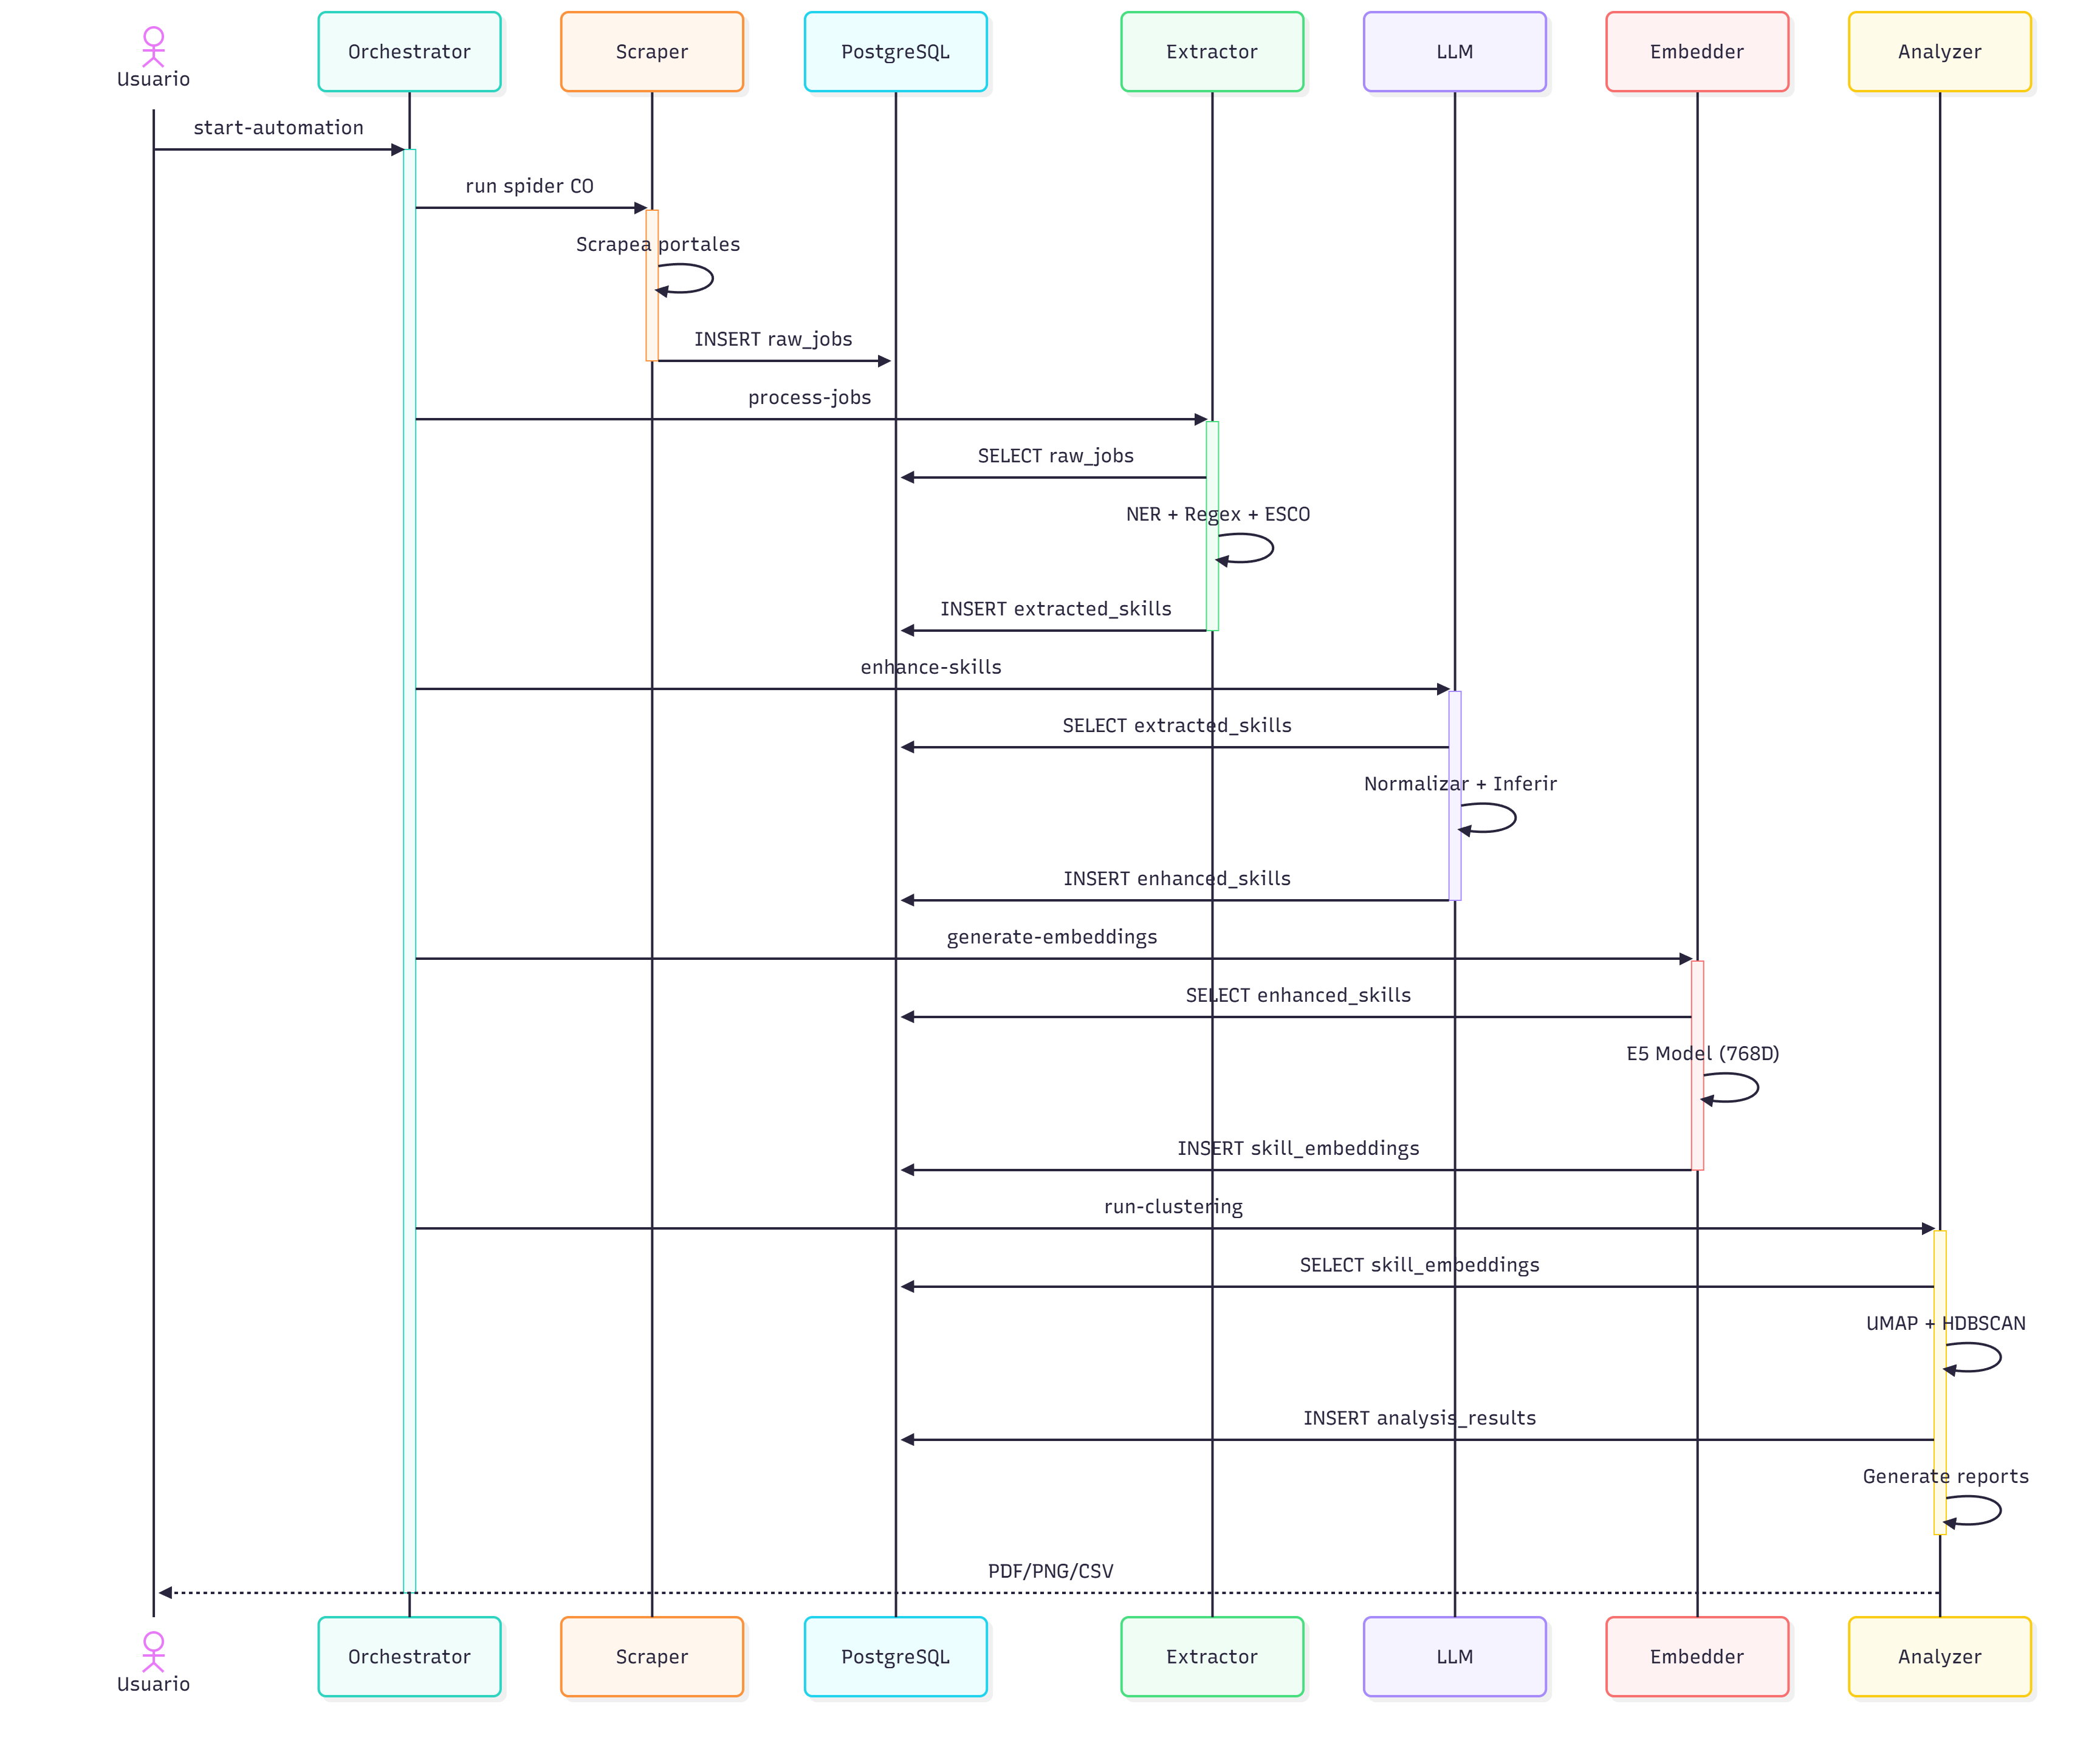
\includegraphics[width=0.95\textwidth]{diagrams/DiagramaSecuencia.png}
\caption{Diagrama de Secuencia de Interacciones del Pipeline Completo}
\label{fig:diagrama-secuencia}
\end{figure}

El flujo de ejecución sigue estos pasos:

\begin{enumerate}
    \item El usuario ejecuta \texttt{start-automation} en el Orchestrator CLI
    \item El Orchestrator lanza el comando \texttt{run spider CO} al módulo Scraper
    \item El Scraper extrae ofertas de los portales web y las inserta en PostgreSQL (\texttt{raw\_jobs})
    \item El Orchestrator ejecuta \texttt{process-jobs}, que activa el Extractor
    \item El Extractor lee ofertas de \texttt{raw\_jobs}, aplica NER + Regex + ESCO, e inserta en \texttt{extracted\_skills}
    \item El Orchestrator ejecuta \texttt{enhance-skills}, que activa el LLM Processor
    \item El LLM lee de \texttt{extracted\_skills}, normaliza e infiere habilidades implícitas, e inserta en \texttt{enhanced\_skills}
    \item El Orchestrator ejecuta \texttt{generate-embeddings}, que activa el Embedder
    \item El Embedder lee de \texttt{enhanced\_skills}, genera vectores 768D con E5 Model, e inserta en \texttt{skill\_embeddings}
    \item El Orchestrator ejecuta \texttt{run-clustering}, que activa el Analyzer
    \item El Analyzer lee de \texttt{skill\_embeddings}, aplica UMAP + HDBSCAN, genera reportes, e inserta resultados en \texttt{analysis\_results}
    \item El Analyzer retorna archivos PDF/PNG/CSV al usuario
\end{enumerate}

Cada paso incluye confirmaciones bidireccionales entre componentes y la base de datos, garantizando consistencia en cada etapa. El manejo de errores permite reintentos en cualquier punto del flujo sin pérdida de datos.

\subsection{Orchestrator CLI}

El sistema se controla mediante un CLI único implementado con Typer:

\begin{verbatim}
python -m src.orchestrator <comando> [opciones]
\end{verbatim}

\textbf{Comandos principales}:
\begin{itemize}
    \item \texttt{run-once <spider> <country>}: Ejecutar scraping único
    \item \texttt{run <spiders> <country>}: Ejecutar múltiples spiders
    \item \texttt{process-jobs}: Procesar ofertas pendientes
    \item \texttt{status}: Estado del sistema y estadísticas
    \item \texttt{health}: Métricas de salud del sistema
    \item \texttt{start-automation}: Iniciar sistema automatizado
    \item \texttt{automation-status}: Estado del scheduler
    \item \texttt{list-jobs}: Listar trabajos programados
\end{itemize}

\subsection{Sistema de Automatización}

Tres componentes coordinan la operación 24/7:

\begin{enumerate}
    \item \textbf{Master Controller}: Coordinador central que gestiona el ciclo de vida del sistema
    \item \textbf{Intelligent Scheduler}: Basado en APScheduler, programa ejecuciones periódicas de spiders con estrategias adaptativas
    \item \textbf{Pipeline Automator}: Detecta nuevos trabajos y los procesa automáticamente a través del pipeline de extracción
\end{enumerate}

\textbf{Programación de spiders}:
\begin{itemize}
    \item Frecuencia configurable por portal (cada 6-12 horas)
    \item Ventanas de ejecución para minimizar detección
    \item Priorización dinámica basada en tasa de actualización del portal
    \item Reintentos automáticos con backoff exponencial
\end{itemize}

\section{Métricas de Evaluación}

\subsection{Métricas por Módulo}

\subsubsection{Scraper}
\begin{itemize}
    \item \textbf{Tasa de éxito}: (peticiones exitosas / peticiones totales) × 100
    \item \textbf{Tasa de parseo}: (trabajos parseados / páginas scrapeadas) × 100
    \item \textbf{Tasa de duplicados}: (trabajos duplicados / trabajos totales) × 100
    \item \textbf{Cobertura}: trabajos únicos por portal por país
\end{itemize}

\subsubsection{Extractor}
\begin{itemize}
    \item \textbf{Precisión}: habilidades validadas / habilidades extraídas
    \item \textbf{Recall}: habilidades extraídas / habilidades anotadas (gold standard)
    \item \textbf{F1-Score}: media armónica de precisión y recall
    \item \textbf{Tasa de mapeo ESCO}: habilidades mapeadas a ESCO / total habilidades
\end{itemize}

\subsubsection{LLM Processor}
\begin{itemize}
    \item \textbf{Tasa de deduplicación}: habilidades deduplicadas / habilidades de entrada
    \item \textbf{Descubrimiento de habilidades implícitas}: habilidades implícitas / total habilidades enriquecidas
    \item \textbf{Éxito de normalización}: habilidades normalizadas con ESCO / total habilidades
    \item \textbf{Tiempo de procesamiento}: tiempo promedio por oferta laboral
\end{itemize}

\subsubsection{Clustering}
\begin{itemize}
    \item \textbf{Silhouette Score}: Medida de cohesión y separación de clústeres (-1 a 1, óptimo $>$ 0.5)
    \item \textbf{Davies-Bouldin Index}: Validez de clústeres (menor es mejor)
    \item \textbf{Estabilidad de clústeres}: Consistencia entre ejecuciones con semillas diferentes
    \item \textbf{Cobertura}: trabajos en clústeres / trabajos totales
\end{itemize}

\subsection{Métricas del Sistema}

\textbf{Métricas de rendimiento}:
\begin{itemize}
    \item Trabajos procesados por hora
    \item Tiempo promedio de extracción por trabajo
    \item Tiempo promedio de procesamiento LLM por trabajo
    \item Tiempo promedio de generación de embedding por habilidad
    \item Latencia de búsqueda de similitud vectorial
\end{itemize}

\textbf{Métricas de calidad}:
\begin{itemize}
    \item F1 Score de extracción de habilidades
    \item Cobertura de enriquecimiento LLM
    \item Silhouette Score de clustering
    \item Tasa de mapeo a ESCO
    \item Consistencia inter-anotadores (para subset validado)
\end{itemize}

\textbf{Objetivo de escala}: El sistema fue diseñado para procesar 600,000 ofertas laborales para la fecha de defensa, con capacidad de crecimiento horizontal mediante:
\begin{itemize}
    \item Particionamiento de tablas por país y fecha
    \item Procesamiento por lotes configurable
    \item Índices optimizados para consultas frecuentes
    \item Caché de embeddings para habilidades recurrentes
\end{itemize}
